\subsection{Best Visualization Configurations}
\label{subsec:best-visualization-configs}

The best visualization configurations for each dataset demonstrate distinct characteristics and optimal parameter settings. For both datasets, we explored various combinations of dimensionality reduction, clustering, and visualization techniques to find the most effective representations.

\begin{figure}[h!]
    \centering
    % First subfigure
    \begin{subfigure}[b]{0.45\textwidth}
        \centering
        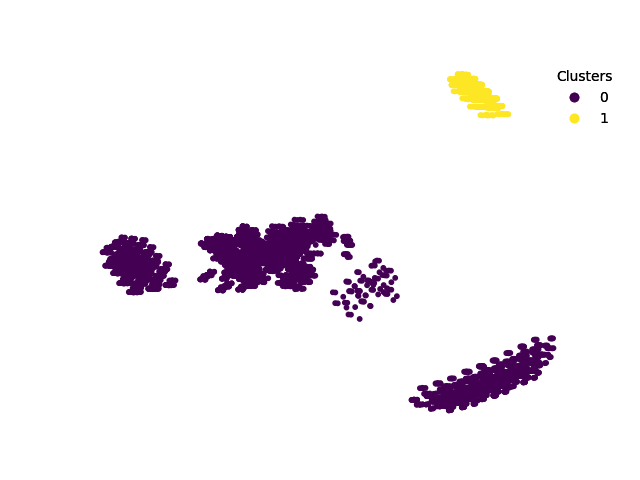
\includegraphics[width=\textwidth]{figures/visualizations/pca_n_components=3,kernel=rbf,gamma=0.1,n_clusters=2,max_iterations=100,tolerance=0.001,random_state=4.png}
        \caption{Mushroom dataset using kernel PCA and global k-means}
        \label{subfig:best_mushroom_viz}
    \end{subfigure}
    \hfill
    % Second subfigure
    \begin{subfigure}[b]{0.45\textwidth}
        \centering
        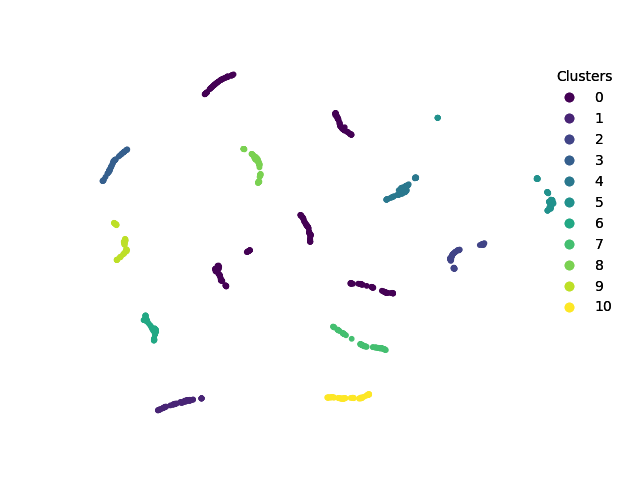
\includegraphics[width=\textwidth]{figures/visualizations/umap_n_components=11,kernel=rbf,gamma=1,n_clusters=11,max_iterations=100,tolerance=0.0001,random_state=4.png}
        \caption{Vowel dataset using UMAP and global k-means}
        \label{subfig:best_vowel_viz}
    \end{subfigure}
    
    \caption{Best visualization configurations for both datasets}
    \label{fig:best_visualizations}
\end{figure}

\paragraph{Mushroom dataset}
For the mushroom dataset (Figure \ref{subfig:best_mushroom_viz}), kernel PCA reduction combined with global k-means clustering produces two well-separated and compact clusters. This configuration uses the following parameters:
\begin{itemize}
    \item PCA: \texttt{n\_components=3}, \texttt{kernel=rbf}, \texttt{gamma=0.1}
    \item Clustering: \texttt{n\_clusters=2}, \texttt{max\_iterations=100}, \texttt{tolerance=0.001}
\end{itemize}

The effectiveness of this configuration stems from kernel PCA's ability to capture non-linear relationships in the categorical features of the mushroom dataset, resulting in clearly separable clusters.

\paragraph{Vowel dataset}
For the vowel dataset (Figure \ref{subfig:best_vowel_viz}), UMAP visualization with kernel PCA reduction and global k-means clustering provides the most interpretable representation. The configuration uses:
\begin{itemize}
    \item UMAP: \texttt{n\_components=11}
    \item Kernel PCA: \texttt{kernel=rbf}, \texttt{gamma=1}
    \item Clustering: \texttt{n\_clusters=11}, \texttt{max\_iterations=100}, \texttt{tolerance=0.0001}
\end{itemize}

While the vowel dataset's clusters appear as lines rather than compact blobs, this configuration effectively captures the dataset's complex structure with its 11 distinct vowel classes. UMAP's ability to preserve both local and global structures makes it particularly suitable for visualizing this high-dimensional dataset with overlapping clusters.
